\chapter{Selección de las Series de Estudio}
\label{chap:seleccionvariable}

La elección de las series temporales para esta investigación no es
arbitraria; se fundamenta en su relevancia para la toma de
decisiones, la disponibilidad de datos históricos consistentes y,
crucialmente, su capacidad para ser modeladas con rigor matemático
\cite{Forecasting2022}.  Indicadores como el Producto Interno Bruto
(PIB) o los precios de combustibles no solo reflejan dinámicas
complejas influenciadas por políticas internas y shocks globales,
sino que ofrecen un campo de pruebas idóneo para validar la robustez
de la metodología TCROC desarrollada en los
Capítulos~\ref{cap:tcroc}--\ref{cap:sec_ssrc}
\cite{EconHonduras, Hamilton1994}.

El presente trabajo se enfoca en dos familias de datos con
características deliberadamente contrastantes: una serie
macroeconómica de baja frecuencia y un conjunto de series de mercado
de alta frecuencia.  Esta dualidad permite evaluar la versatilidad y
precisión del marco TCROC-Markov en contextos fundamentalmente
distintos \cite{kolassa2023, Tsay2005}.

% ===================================================================
\section{El PIB de Honduras como Serie Macroeconómica}
\label{sec:pib_serie}
% ===================================================================

El Producto Interno Bruto es el indicador canónico para medir la
salud y el crecimiento de una economía.  Su análisis es fundamental
para entender las tendencias a largo plazo y el impacto de eventos
estructurales, como crisis políticas o sanitarias.  Para este
estudio se utilizan cuatro variantes del PIB de Honduras, con un
enfoque en el período 2000--2023 para los análisis cuantitativos,
aunque se presentan los gráficos históricos completos desde 1960.

\subsection{PIB en dólares corrientes}

El PIB a precios corrientes de mercado es la medida más amplia de la
producción económica de un país \cite{WorldBankGDP}.  Su evolución,
mostrada en la Figura~\ref{fig:PIBHNVal01}, ilustra la trayectoria
de crecimiento nominal de la economía hondureña a lo largo de más de
seis décadas.

\begin{figure}[H]
\centering
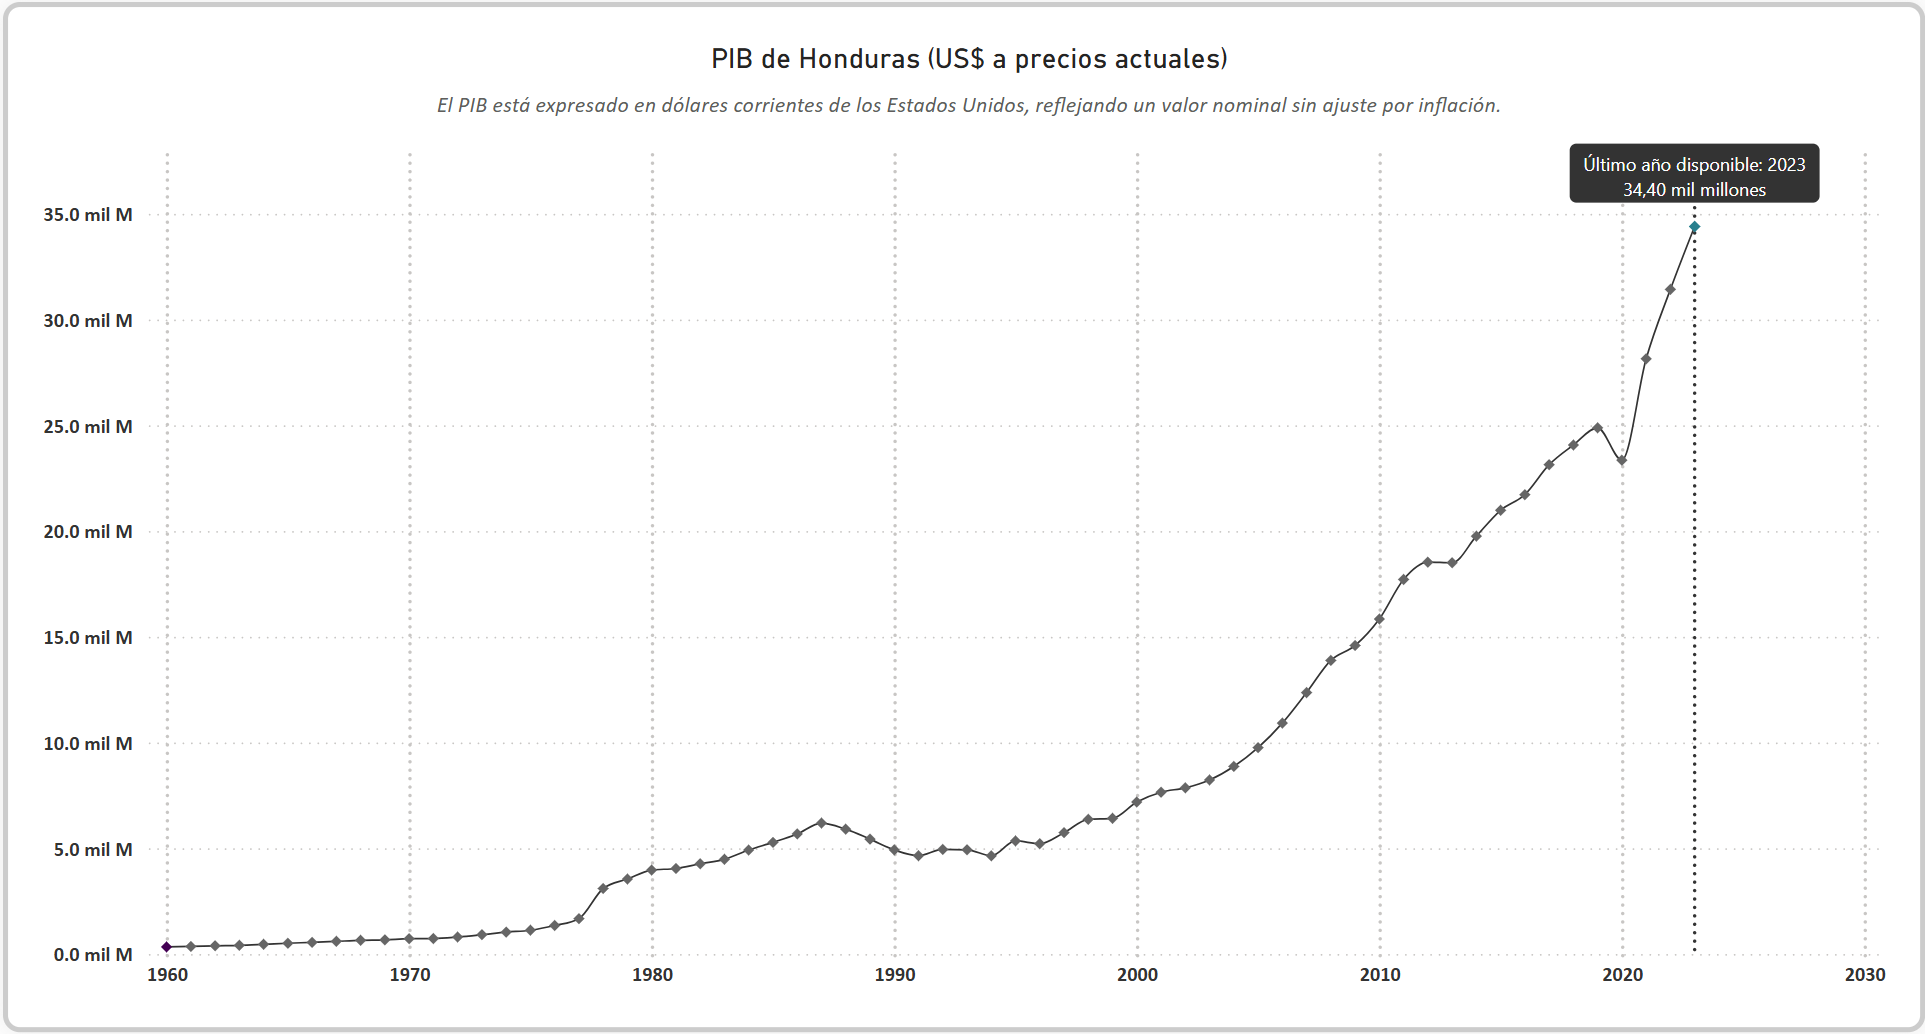
\includegraphics[width=0.85\textwidth]{figures/PIBHNVal.png}
\caption{Evolución del PIB de Honduras en dólares corrientes,
1960--2023.  Fuente:~\cite{WorldBankGDP}.}
\label{fig:PIBHNVal01}
\end{figure}

\subsection{Tasa de crecimiento anual del PIB}

La tasa de crecimiento real del PIB, ajustada por inflación, revela
períodos de expansión y recesión \cite{WorldBankGDPGrowth}.  La
Figura~\ref{fig:PIBHNPer01} expone la volatilidad de este indicador,
con caídas pronunciadas en 2009 y 2020.

\begin{figure}[H]
\centering
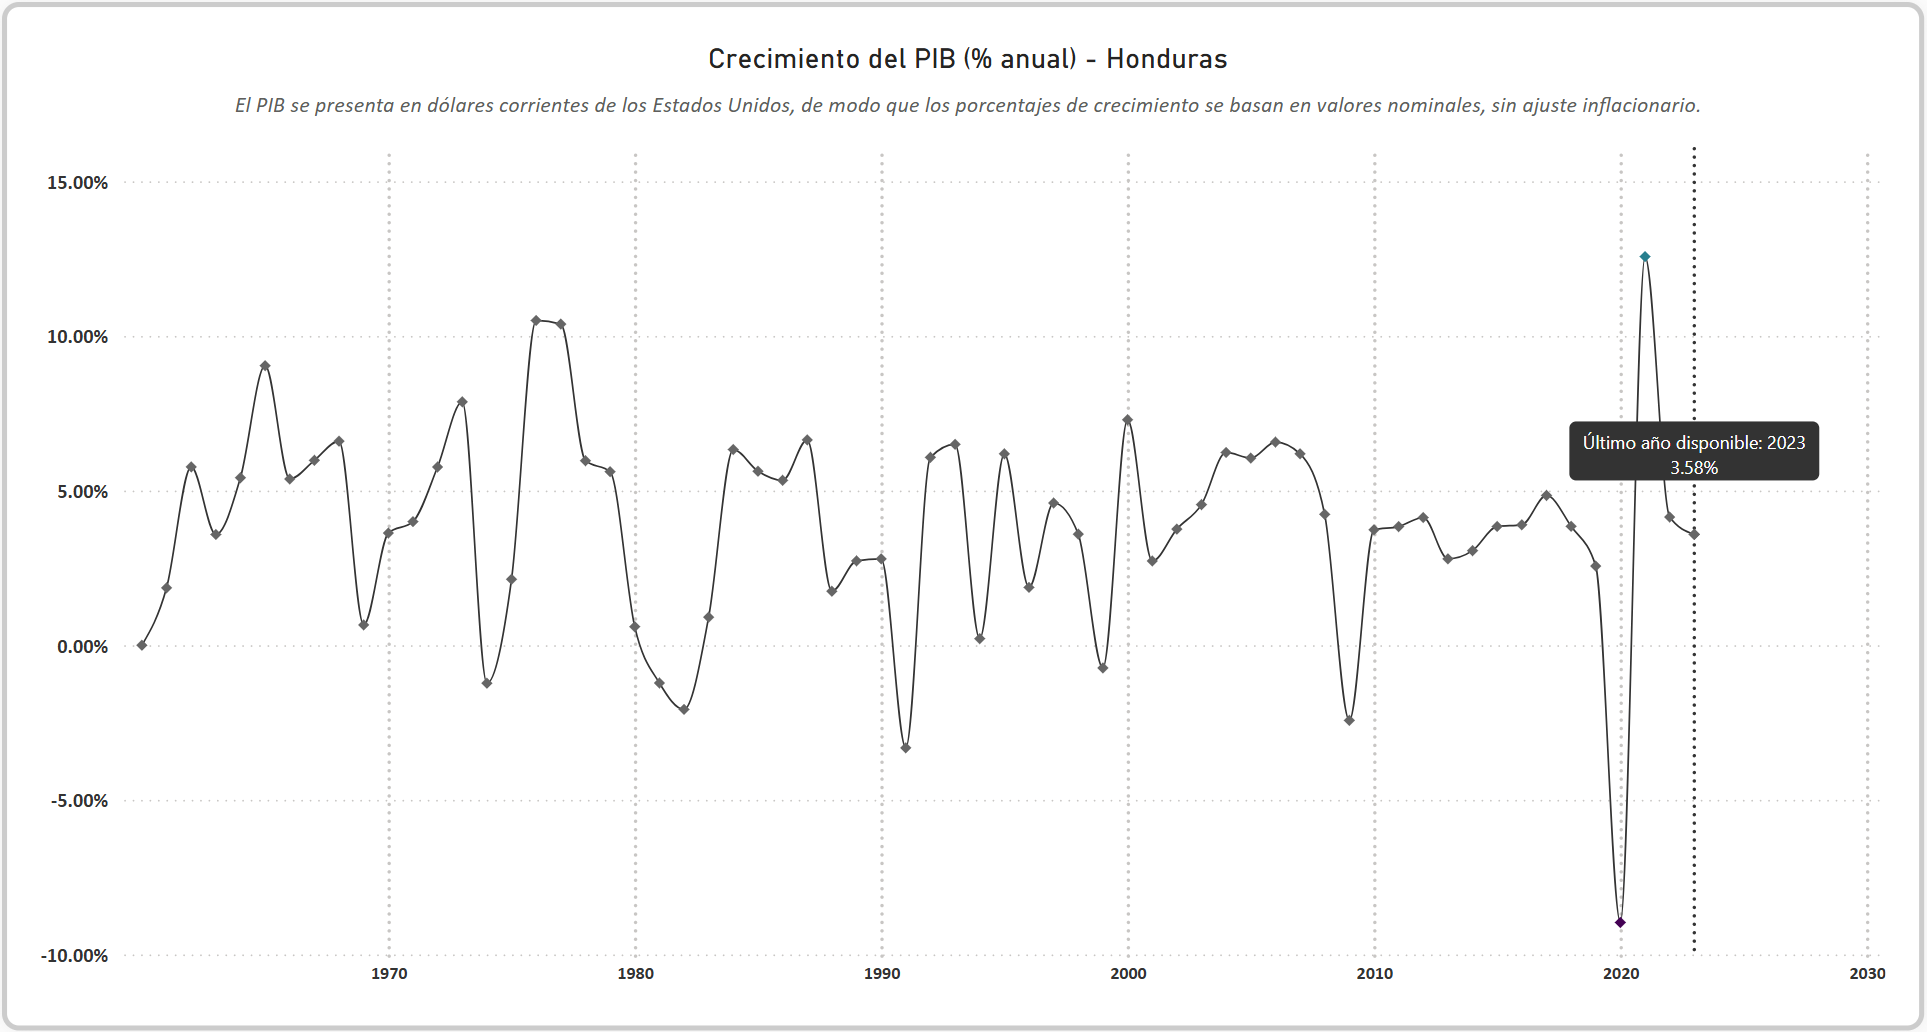
\includegraphics[width=0.85\textwidth]{figures/PIBHNPer.png}
\caption{Tasa de crecimiento anual del PIB de Honduras,
1961--2023.  Fuente:~\cite{WorldBankGDPGrowth}.}
\label{fig:PIBHNPer01}
\end{figure}

\subsection{PIB per cápita en dólares corrientes}

El PIB per cápita ofrece una aproximación a la prosperidad promedio y
al nivel de vida \cite{WorldBankGDPPC}.  Su trayectoria, visible en
la Figura~\ref{fig:PIBHNCap01}, es fundamental para evaluar el
desarrollo económico en términos humanos.

\begin{figure}[H]
\centering
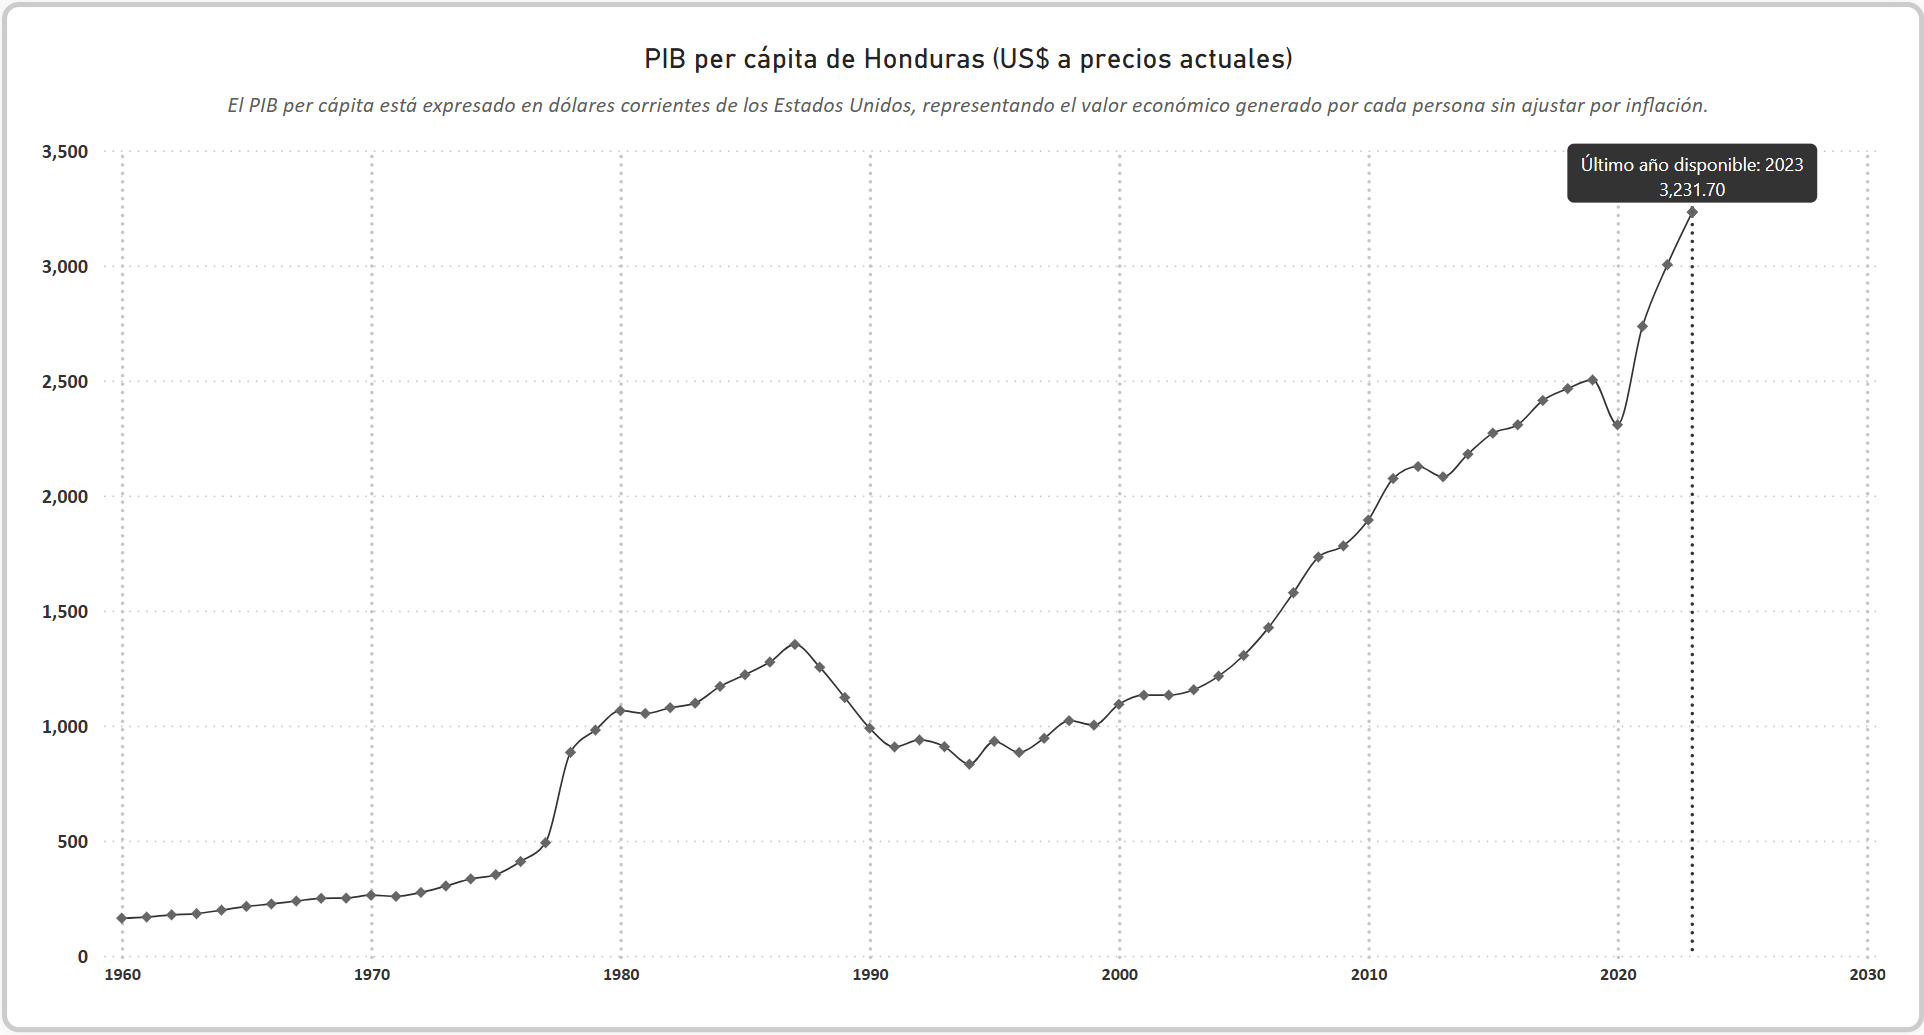
\includegraphics[width=0.9\textwidth]{figures/PIBHNCap.png}
\caption{PIB per cápita de Honduras en dólares corrientes,
1960--2023.  Fuente:~\cite{WorldBankGDPPC}.}
\label{fig:PIBHNCap01}
\end{figure}

\subsection{PIB per cápita en lempiras a precios constantes}

Esta es la serie de referencia principal para los análisis de los
Capítulos~\ref{cap:tcroc} y~\ref{cap:tcroc_hibrido_integrado}.
Al estar denominada en moneda local y a precios constantes, elimina
los efectos tanto de la inflación como de las fluctuaciones del tipo
de cambio, ofreciendo la medida más pura de la producción real por
habitante \cite{WorldBankGDPPCConst}.

\begin{figure}[H]
\centering
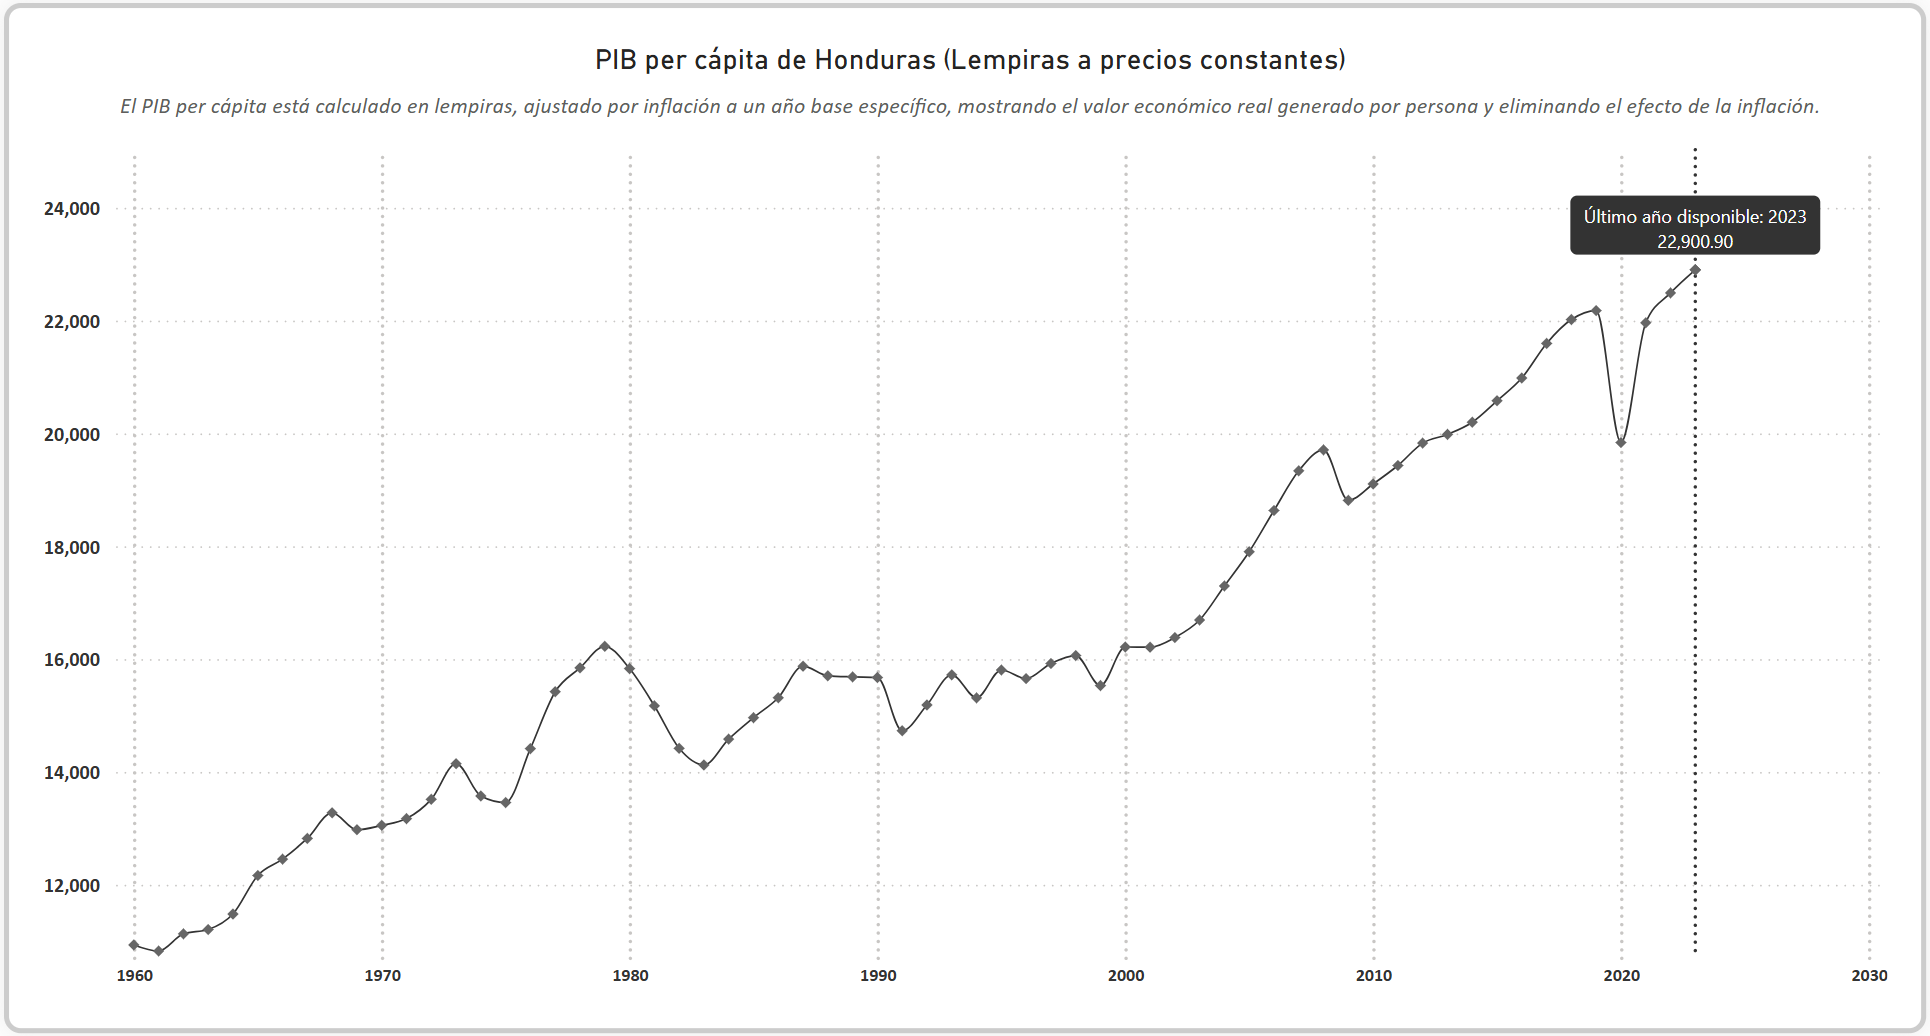
\includegraphics[width=0.9\textwidth]{figures/PIBHNCapConst.png}
\caption{PIB per cápita de Honduras en lempiras a precios
constantes, 1960--2023.  Fuente:~\cite{WorldBankGDPPCConst}.}
\label{fig:PIBHNCapConst01}
\end{figure}

La Tabla~\ref{tbl:SeriesEvolution} resume numéricamente la evolución
de estas series para el período de estudio principal (2000--2023),
que sirve de base para la estimación de los modelos.

\begin{table}[H]
\centering
\caption{Evolución de series económicas seleccionadas de Honduras,
2000--2023.}
\label{tbl:SeriesEvolution}
\resizebox{\textwidth}{!}{%
\begin{tabular}{|c|r|r|r|r|}
\hline
\textbf{Año} & \textbf{PIB Dólares Corr.\ (M\,USD)} &
\textbf{Crec.\ Anual (\%)} &
\textbf{PIB p.c.\ Dólares (USD)} &
\textbf{PIB p.c.\ Lempiras Const.} \\ \hline
2000 & 7\,186\,638\,029 & 7.29 & 1\,092.6 & 16\,214.3 \\
2001 & 7\,651\,162\,302 & 2.72 & 1\,132.2 & 16\,211.7 \\
2002 & 7\,858\,255\,413 & 3.75 & 1\,132.5 & 16\,381.9 \\
2003 & 8\,230\,391\,347 & 4.55 & 1\,156.1 & 16\,692.9 \\
2004 & 8\,869\,299\,234 & 6.23 & 1\,215.1 & 17\,296.5 \\
2005 & 9\,757\,012\,697 & 6.05 & 1\,304.7 & 17\,903.1 \\
2006 & 10\,917\,477\,066 & 6.57 & 1\,425.8 & 18\,634.1 \\
2007 & 12\,361\,257\,681 & 6.19 & 1\,577.7 & 19\,337.8 \\
2008 & 13\,881\,731\,876 & 4.23 & 1\,732.5 & 19\,708.9 \\
2009 & 14\,587\,496\,229 & $-2.43$ & 1\,781.2 & 18\,813.3 \\
2010 & 15\,839\,344\,592 & 3.73 & 1\,893.3 & 19\,104.7 \\
2011 & 17\,710\,275\,685 & 3.84 & 2\,073.7 & 19\,431.7 \\
2012 & 18\,528\,554\,398 & 4.13 & 2\,126.0 & 19\,828.9 \\
2013 & 18\,499\,729\,215 & 2.79 & 2\,081.1 & 19\,983.0 \\
2014 & 19\,756\,533\,972 & 3.06 & 2\,179.9 & 20\,199.1 \\
2015 & 20\,979\,791\,685 & 3.84 & 2\,271.2 & 20\,579.2 \\
2016 & 21\,717\,604\,952 & 3.89 & 2\,307.3 & 20\,982.7 \\
2017 & 23\,136\,247\,991 & 4.84 & 2\,413.0 & 21\,595.6 \\
2018 & 24\,067\,750\,760 & 3.84 & 2\,464.6 & 22\,019.3 \\
2019 & 24\,882\,225\,742 & 2.56 & 2\,502.3 & 22\,177.7 \\
2020 & 23\,352\,232\,484 & $-8.97$ & 2\,307.6 & 19\,838.3 \\
2021 & 28\,144\,331\,507 & 12.57 & 2\,735.1 & 21\,961.6 \\
2022 & 31\,426\,041\,807 & 4.14 & 3\,003.3 & 22\,491.3 \\
2023 & 34\,400\,509\,852 & 3.58 & 3\,231.7 & 22\,900.9 \\
\hline
\end{tabular}%
}
\end{table}

% ===================================================================
\section[Precios de Combustibles]{Precios de Combustibles como Serie
de Alta Frecuencia}
\label{sec:combustibles_serie}
% ===================================================================

Para contrastar la dinámica macroeconómica de baja frecuencia del
PIB, se analiza un conjunto de series de mercado de alta frecuencia:
los precios semanales de los combustibles en Honduras.  Estas series
son particularmente valiosas porque reflejan de manera casi
instantánea las volatilidades de los mercados internacionales y las
políticas de precios locales.  Los datos, que abarcan desde
\textbf{2017 hasta 2025}, fueron construidos para esta investigación
mediante un meticuloso proceso de \textit{web scraping} del portal
Proceso Digital \cite{ProcesoHN2025}, seguido de una rigurosa
limpieza y estructuración.  Estas series constituyen el banco de
pruebas empírico del
Capítulo~\ref{cap:regimenes_combustibles}.

\subsection{Precio de la Gasolina Superior}

La evolución del precio de la gasolina superior es un indicador
sensible tanto a los precios internacionales del crudo como a la
demanda interna.

\begin{figure}[H]
\centering
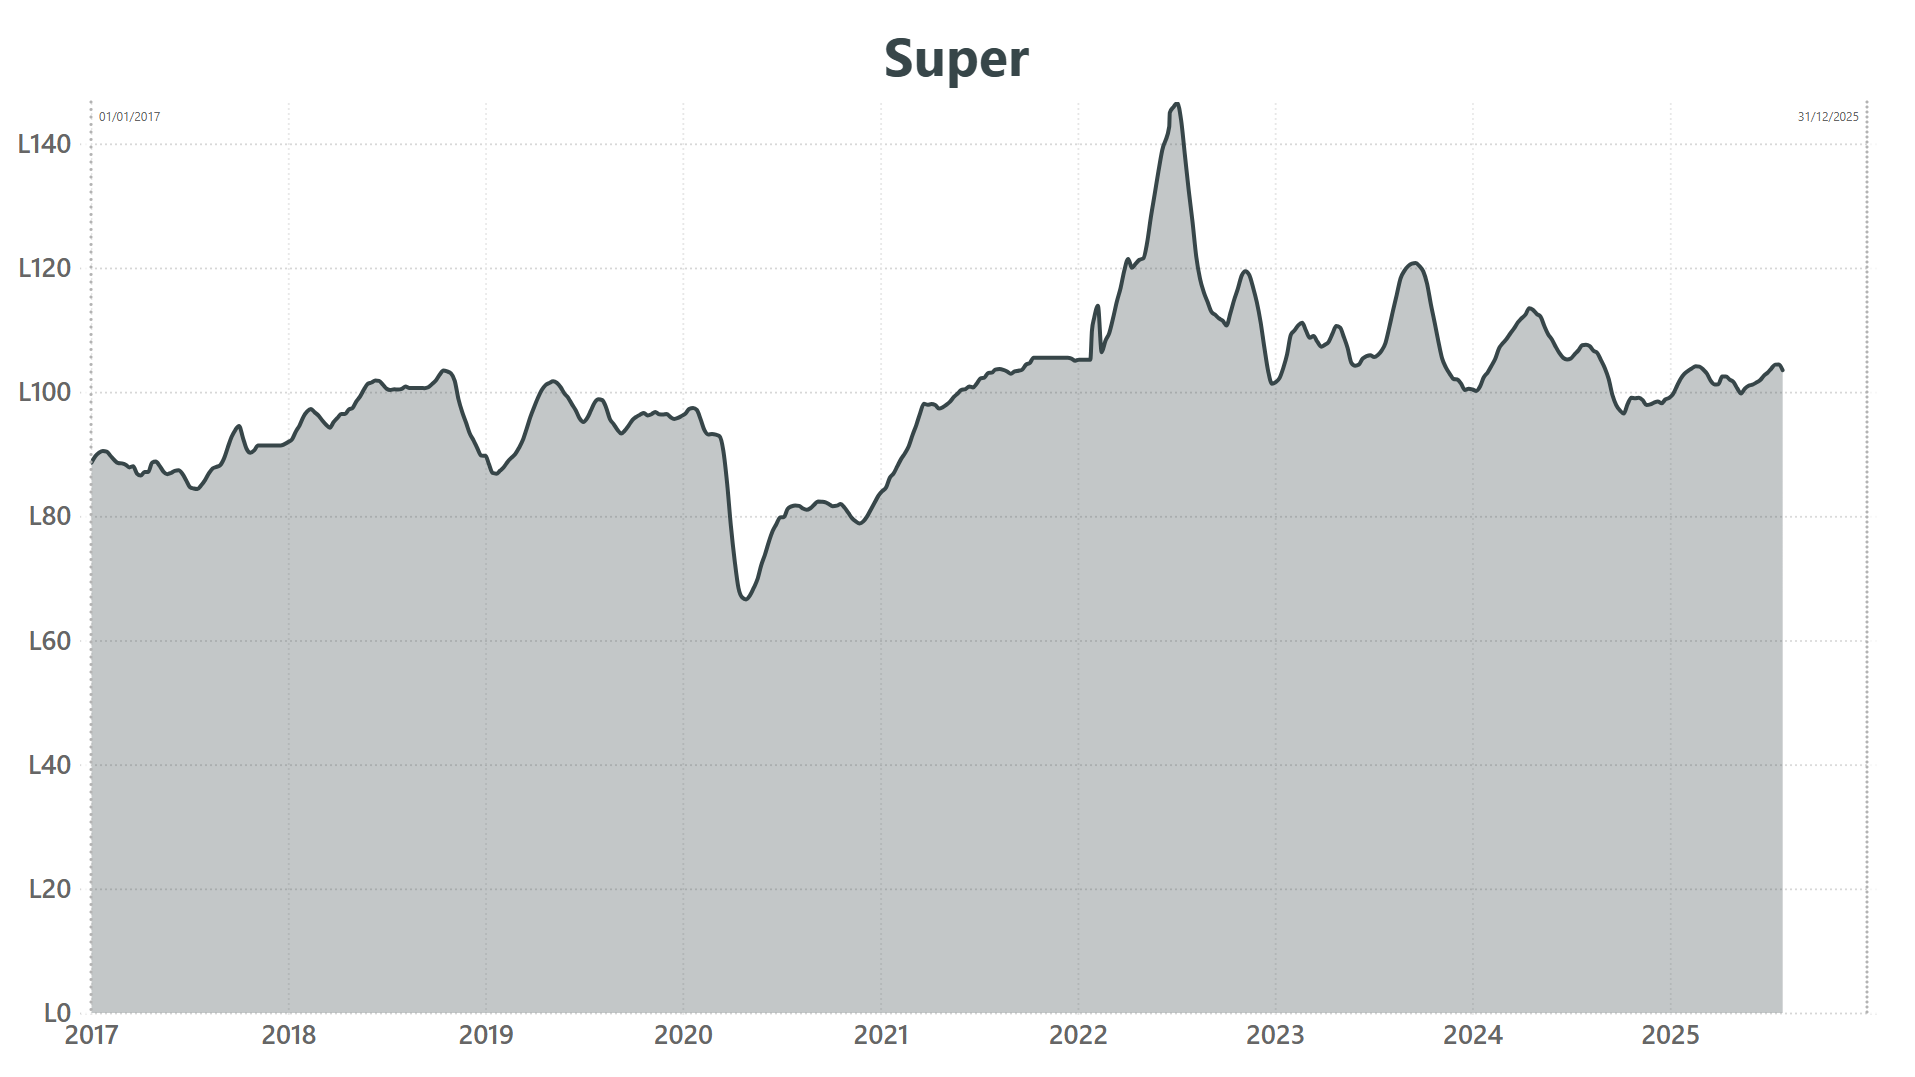
\includegraphics[width=0.95\textwidth]{figures/precio_super.png}
\caption{Precio semanal de la gasolina Superior en Honduras.}
\label{fig:precio_super}
\end{figure}

\subsection{Precio de la Gasolina Regular}

Siendo el combustible de mayor consumo, su precio tiene un impacto
directo en el costo de transporte y, por ende, en la inflación al
consumidor.

\begin{figure}[H]
\centering
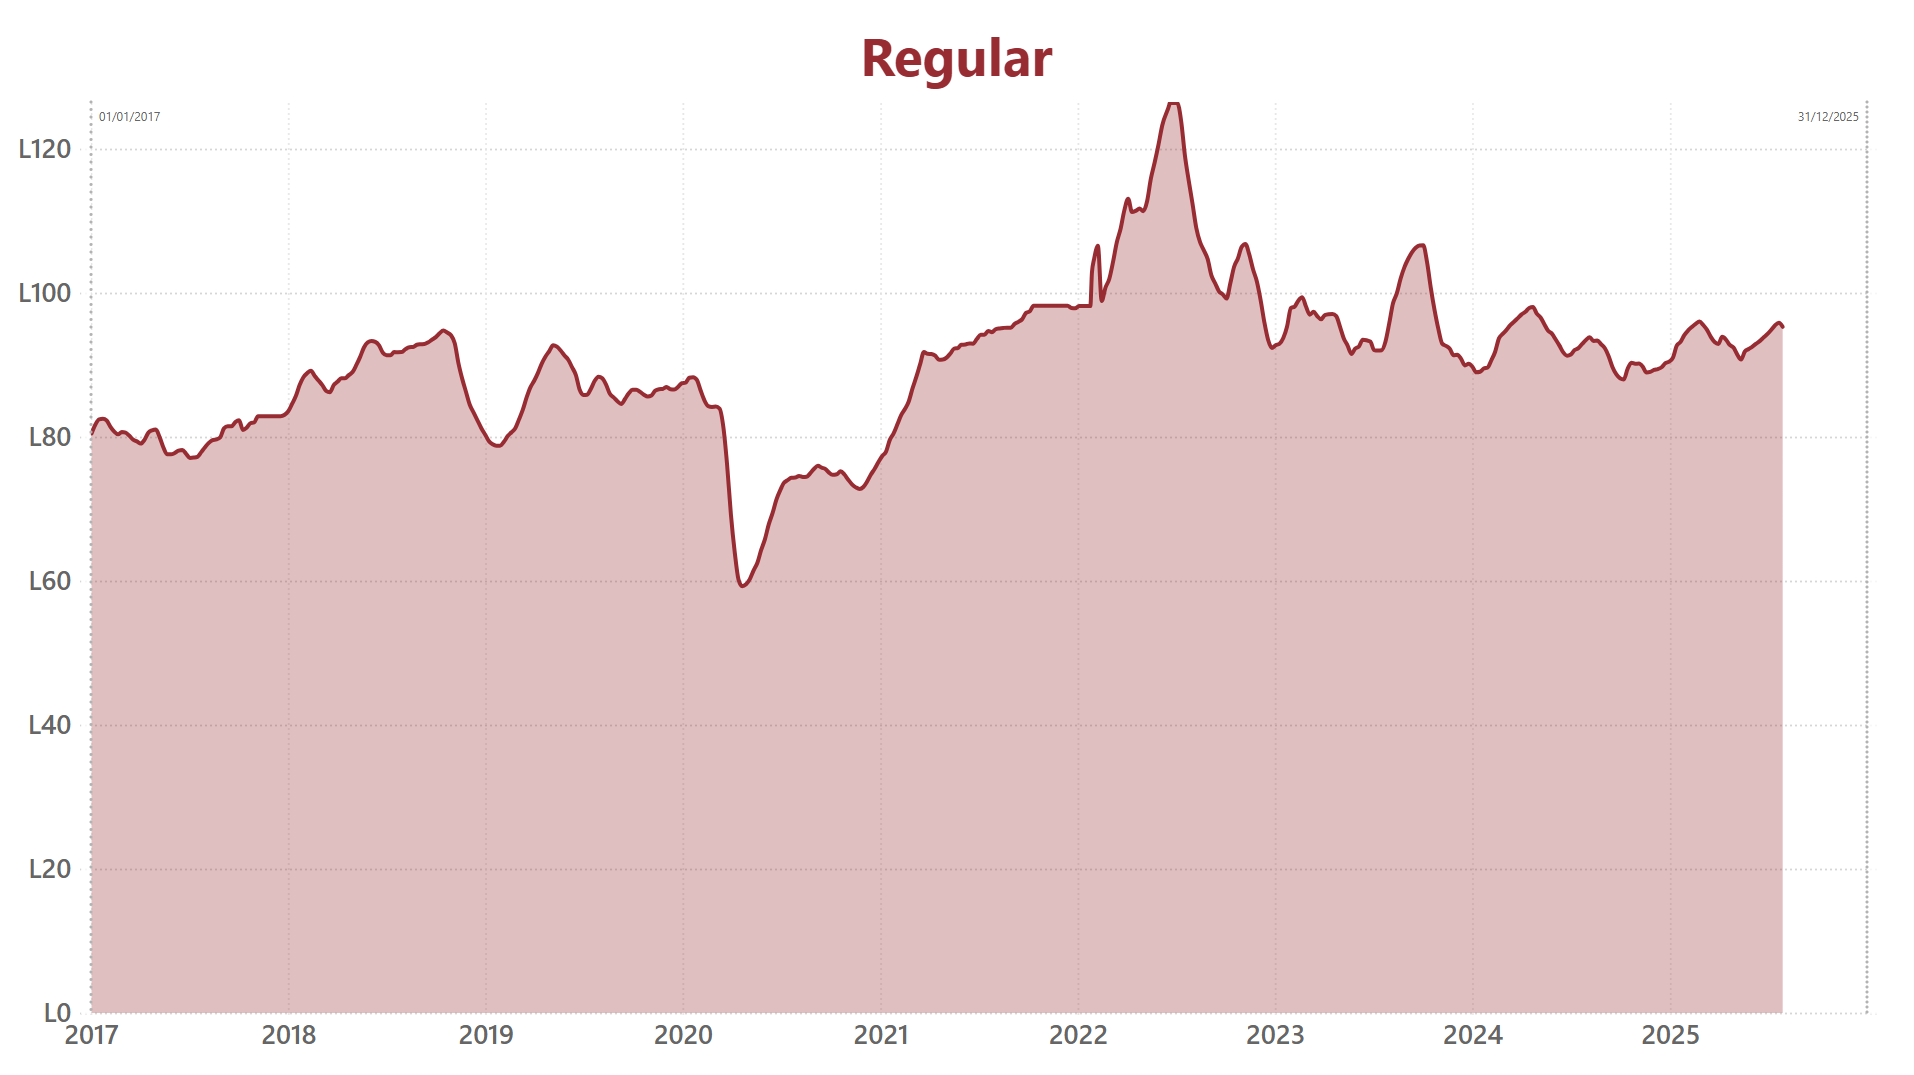
\includegraphics[width=0.95\textwidth]{figures/precio_regular.png}
\caption{Precio semanal de la gasolina Regular en Honduras.}
\label{fig:precio_regular}
\end{figure}

\subsection{Precio del Diésel}

El diésel es fundamental para el transporte de carga y la industria,
por lo que sus fluctuaciones afectan directamente los costos de
producción y la cadena de suministro del país.

\begin{figure}[H]
\centering
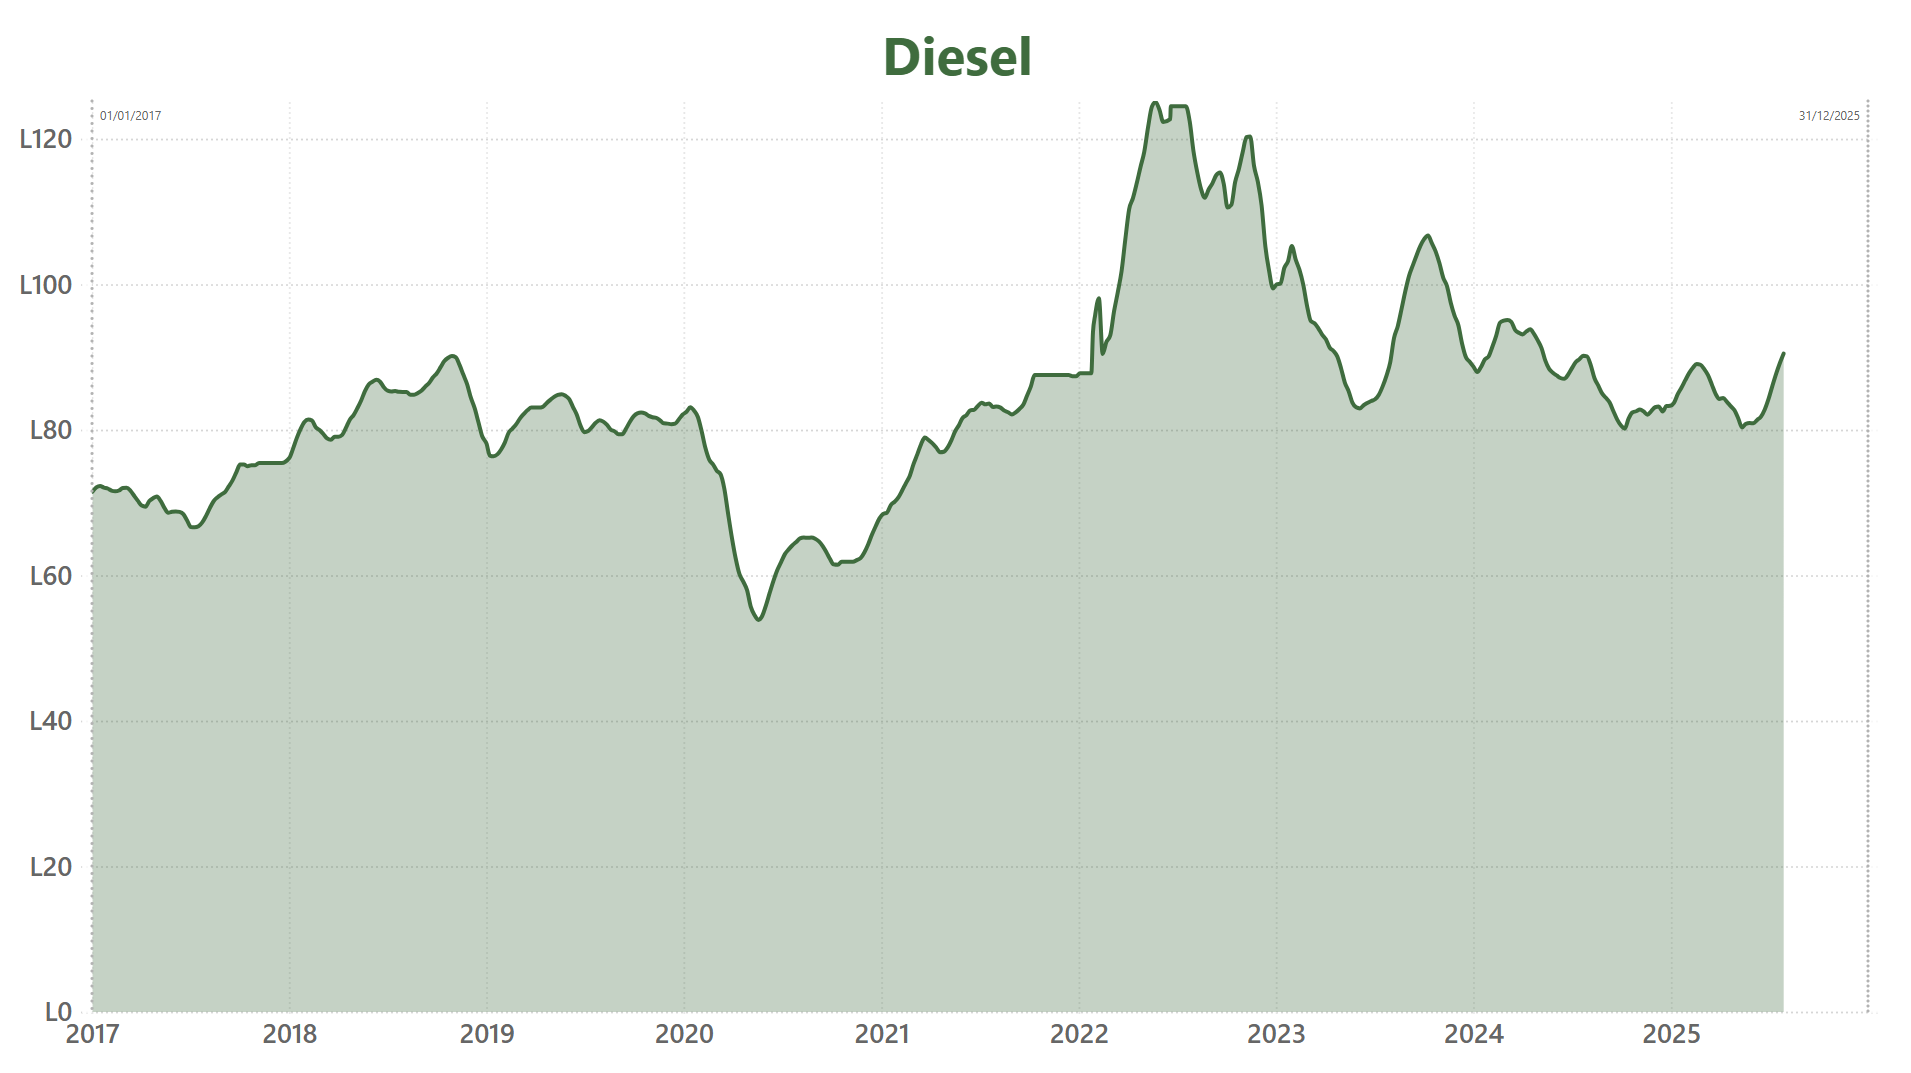
\includegraphics[width=0.95\textwidth]{figures/precio_diesel.png}
\caption{Precio semanal del Diésel en Honduras.}
\label{fig:precio_diesel}
\end{figure}

\subsection{Precio del Kerosene}

Utilizado principalmente para fines domésticos en zonas rurales, el
precio del kerosene es un indicador con importantes implicaciones
sociales.

\begin{figure}[H]
\centering
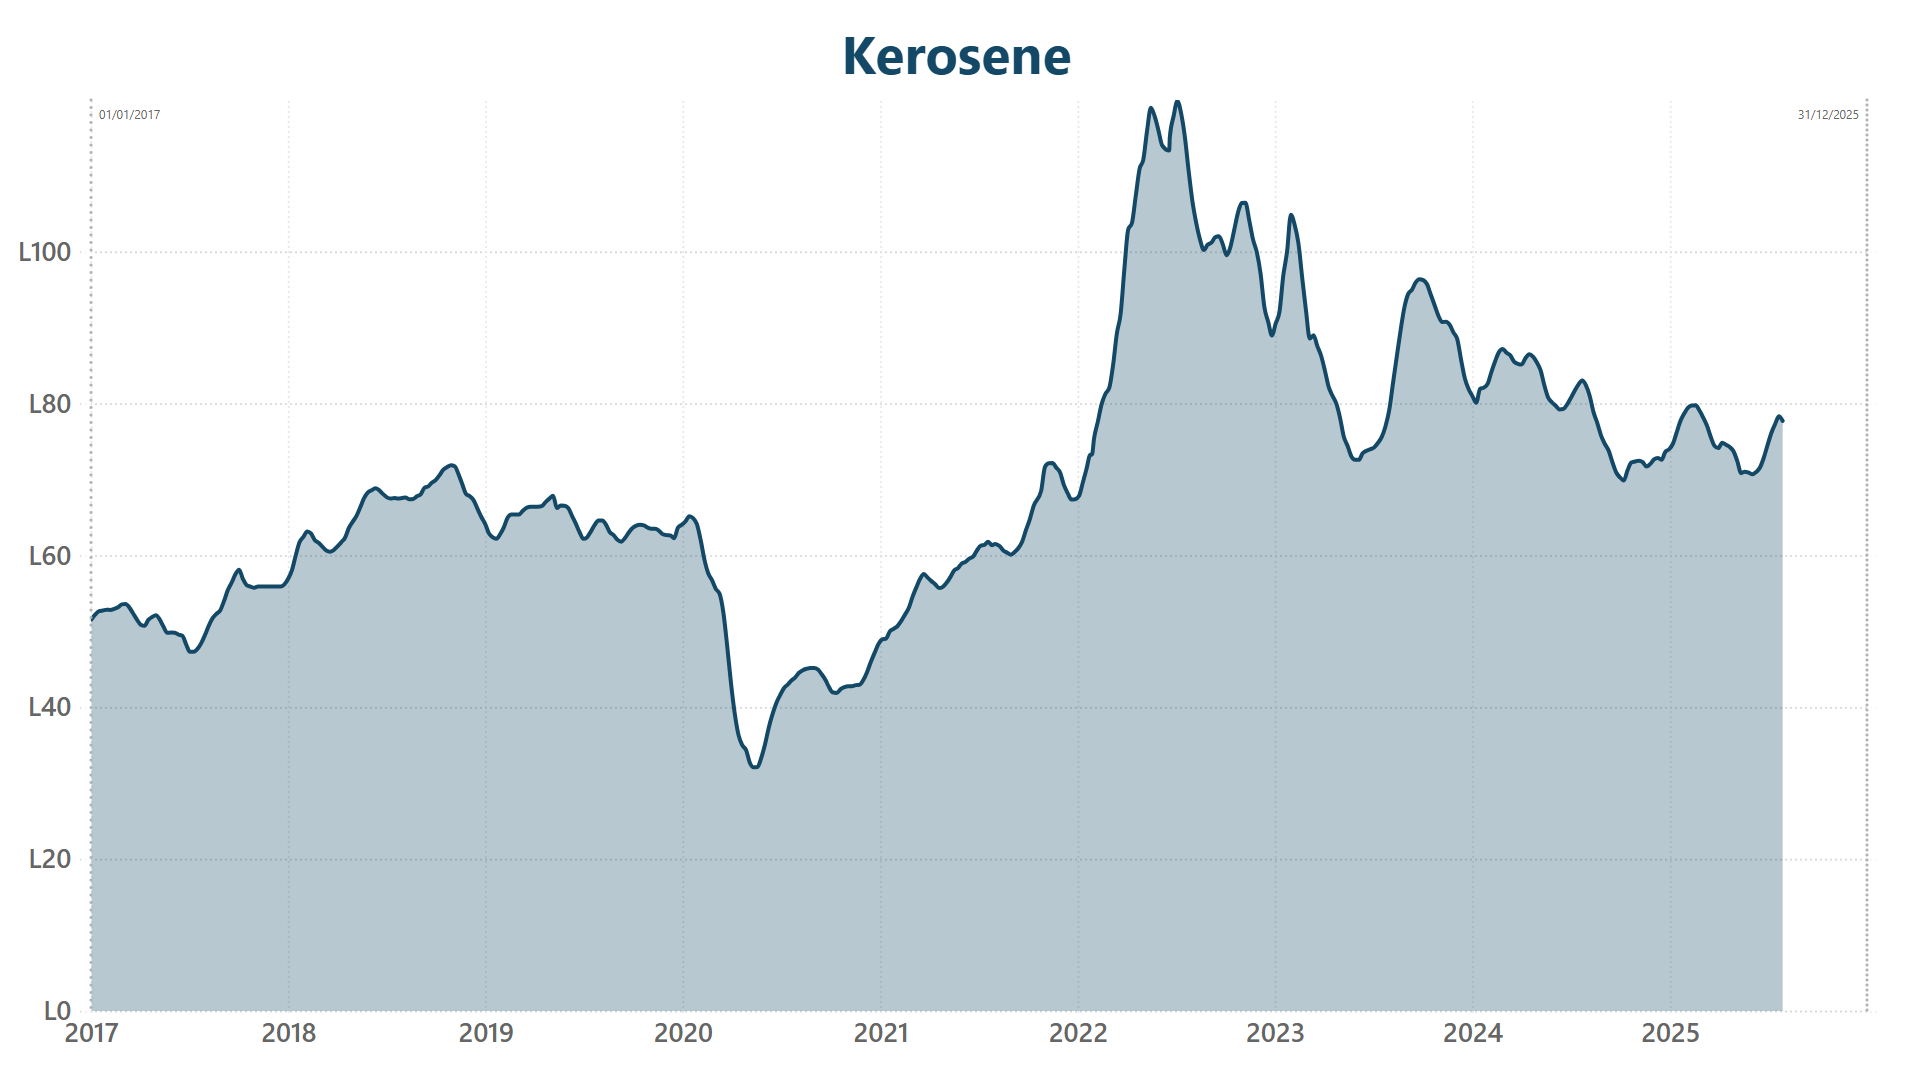
\includegraphics[width=0.95\textwidth]{figures/precio_kerosene.png}
\caption{Precio semanal del Kerosene en Honduras.}
\label{fig:precio_kerosene}
\end{figure}

En conclusión, la elección de estas dos familias de series ---el PIB
como indicador macroeconómico estructural y los combustibles como
indicadores de mercado volátiles--- proporciona un campo de pruebas
diverso y robusto.  Esta dualidad permite validar la eficacia del
modelo TCROC y sus extensiones estocásticas para capturar dinámicas
económicas fundamentalmente distintas, demostrando su versatilidad y
aplicabilidad general.
